% Options for packages loaded elsewhere
\PassOptionsToPackage{unicode}{hyperref}
\PassOptionsToPackage{hyphens}{url}
\documentclass[
  11pt]{article}
\usepackage{xcolor}
\usepackage{amsmath,amssymb}
\setcounter{secnumdepth}{-\maxdimen} % remove section numbering
\usepackage{iftex}
\ifPDFTeX
  \usepackage[T1]{fontenc}
  \usepackage[utf8]{inputenc}
  \usepackage{textcomp} % provide euro and other symbols
\else % if luatex or xetex
  \usepackage{unicode-math} % this also loads fontspec
  \defaultfontfeatures{Scale=MatchLowercase}
  \defaultfontfeatures[\rmfamily]{Ligatures=TeX,Scale=1}
\fi
\usepackage{lmodern}
\ifPDFTeX\else
  % xetex/luatex font selection
\fi
% Use upquote if available, for straight quotes in verbatim environments
\IfFileExists{upquote.sty}{\usepackage{upquote}}{}
\IfFileExists{microtype.sty}{% use microtype if available
  \usepackage[]{microtype}
  \UseMicrotypeSet[protrusion]{basicmath} % disable protrusion for tt fonts
}{}
\makeatletter
\@ifundefined{KOMAClassName}{% if non-KOMA class
  \IfFileExists{parskip.sty}{%
    \usepackage{parskip}
  }{% else
    \setlength{\parindent}{0pt}
    \setlength{\parskip}{6pt plus 2pt minus 1pt}}
}{% if KOMA class
  \KOMAoptions{parskip=half}}
\makeatother
\usepackage{graphicx}
\makeatletter
\newsavebox\pandoc@box
\newcommand*\pandocbounded[1]{% scales image to fit in text height/width
  \sbox\pandoc@box{#1}%
  \Gscale@div\@tempa{\textheight}{\dimexpr\ht\pandoc@box+\dp\pandoc@box\relax}%
  \Gscale@div\@tempb{\linewidth}{\wd\pandoc@box}%
  \ifdim\@tempb\p@<\@tempa\p@\let\@tempa\@tempb\fi% select the smaller of both
  \ifdim\@tempa\p@<\p@\scalebox{\@tempa}{\usebox\pandoc@box}%
  \else\usebox{\pandoc@box}%
  \fi%
}
% Set default figure placement to htbp
\def\fps@figure{htbp}
\makeatother
\setlength{\emergencystretch}{3em} % prevent overfull lines
\providecommand{\tightlist}{%
  \setlength{\itemsep}{0pt}\setlength{\parskip}{0pt}}
\usepackage[]{natbib}
\bibliographystyle{plainnat}
\usepackage{bookmark}
\IfFileExists{xurl.sty}{\usepackage{xurl}}{} % add URL line breaks if available
\urlstyle{same}
% fallback for those not using the hyperref driver hyperxmp:
\makeatletter
\@ifundefined{xmpquote}{\newcommand{\xmpquote}[1]{#1}}{}
\makeatother
\hypersetup{
  pdftitle={ARDRONICS: reproducible gel-image analysis and in-silico 16S restriction-profile matching},
  hidelinks,
  pdfcreator={LaTeX via pandoc}}

\title{ARDRONICS: reproducible gel-image analysis and in-silico 16S
restriction-profile matching}
\author{Aaron L. Feller$^{1}$\\[2pt] Hinsby Cadillo-Quiroz$^{2}$\\[4pt]
\small $^{1}$Interdisciplinary Life Sciences Graduate Programs,\\
\small The University of Texas at Austin, Austin, Texas, USA\\
\small $^{2}$School of Life Sciences, Arizona State University, Tempe, Arizona, USA}
\date{19 November 2026}

\begin{document}
\maketitle

\section{Summary}\label{summary}

Amplified ribosomal DNA restriction analysis (ARDRA) distinguishes
microorganisms by comparing DNA fragment patterns produced when
restriction enzymes cut an amplified ribosomal RNA gene. ARDRONICS is an
open-source Python pipeline that connects gel-image interpretation with
this comparison. It detects lanes and bands at native image resolution,
estimates fragment sizes from one or two molecular-weight ladders,
records densitometry values, simulates restriction digests from 16S
reference sequences, and ranks reference profiles using one-to-one band
matching and Jaccard distances. It also supports multiple-enzyme
consensus, positive-control checks, and explicit reporting of ambiguous
matches.

The software provides a command-line interface, JSON experiment
configuration, lane-map CSV files, quality-control overlays, tidy CSV
outputs, dendrograms, and an HTML report. ARDRONICS is designed for
researchers who need an inspectable and reproducible bridge between gel
documentation and sequence-derived ARDRA libraries, without requiring a
trained vision model or proprietary gel-analysis software.

\section{Statement of need}\label{statement-of-need}

ARDRA remains useful for low-cost isolate screening and comparison of
microbial communities, but its computational workflow often spans
separate tasks: measuring bands on an image, estimating molecular sizes,
generating theoretical restriction profiles, and comparing patterns.
Manual transcription can introduce lane and size errors, while custom
scripts frequently encode particular primer sets, directory layouts, or
enzyme combinations. A sizing library alone cannot resolve these
problems: pixel migration is not interchangeable with base-pair length,
and references lacking primer-defined ends have uncertain terminal
fragments.

ARDRONICS addresses this gap by preserving experimental metadata and
uncertainty throughout the analysis. Users specify ladder identities,
lane roles, digest enzymes, PCR primers, and reference FASTA sequences.
The software fails loudly on ladder-count mismatches, supports manual
coordinate review, marks unclipped references separately, and identifies
tied or incomplete matches. These choices are intended to make ARDRA
results easier to audit and reproduce rather than to hide measurement
uncertainty behind a single organism label.

\section{State of the field}\label{state-of-the-field}

General-purpose tools such as ImageJ can measure gel bands
\citep{schneider2012imagej}, and GelJ provides DNA-fingerprint image
analysis and comparison \citep{heras2015gelj}. Instrument-associated
packages and commercial suites provide additional gel-documentation
workflows. Sequence tools such as EMBOSS \texttt{restrict}
\citep{rice2000emboss} and Biopython's restriction implementation
\citep{cock2009biopython} can generate theoretical digest products, but
they do not connect those products to native gel images and experimental
lane metadata.

ARDRONICS combines these steps in a Python-native workflow. Its distinct
contribution is not a new restriction-site algorithm or a general image
editor; it is the explicit linkage of reviewed gel coordinates, single-
or dual-ladder calibration, primer-aware 16S library generation,
one-to-one tolerant band assignment, multi-enzyme consensus, and control
validation. This integrated design also distinguishes it from fitting a
black-box image classifier: every intermediate profile and calibration
remains available for inspection.

\section{Software design}\label{software-design}

ARDRONICS uses OpenCV and NumPy for image arrays
\citep{bradski2000opencv, harris2020numpy}, SciPy for peak detection,
interpolation, optimization, and clustering \citep{virtanen2020scipy},
pandas for tidy tabular exchange \citep{mckinney2010pandas}, and
Matplotlib for dendrograms \citep{hunter2007matplotlib}. The
architecture separates gel analysis, in-silico digestion, lane
manifests, profile I/O, matching, and reporting.

\begin{figure}
\centering
\pandocbounded{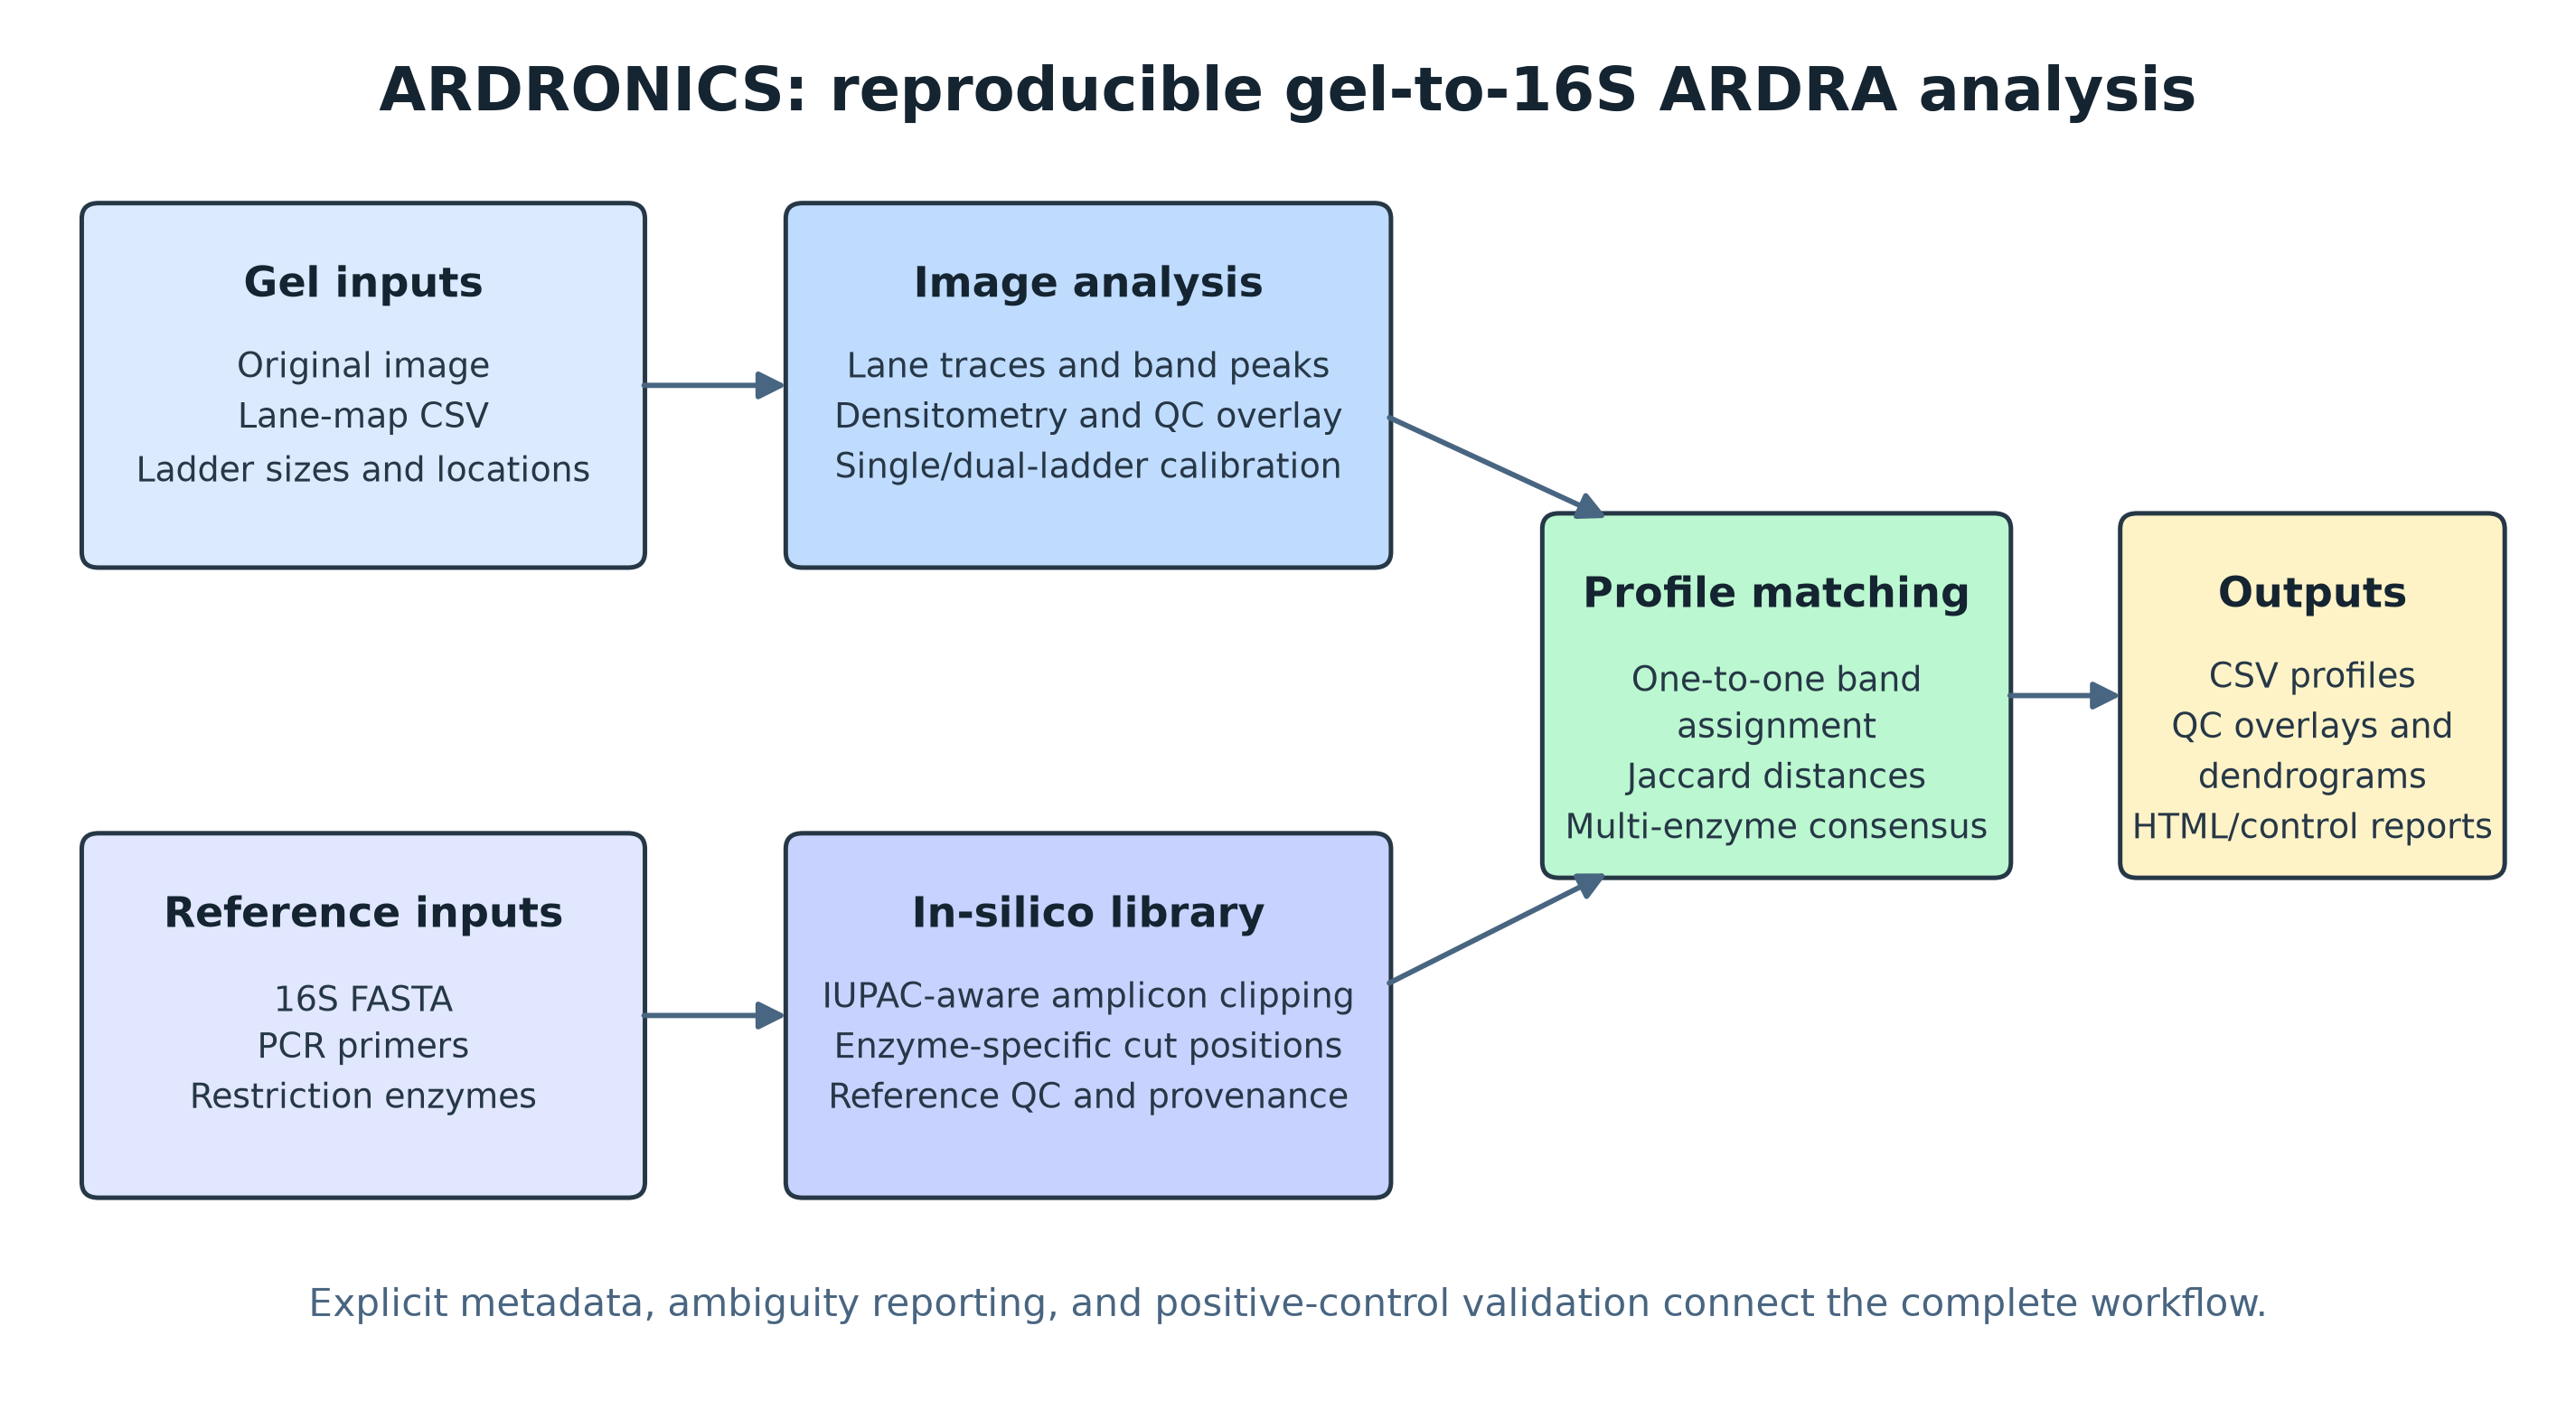
\includegraphics[keepaspectratio,alt={The ARDRONICS
workflow connects reviewed experimental inputs to gel profiles,
theoretical libraries, matching, and quality-control
outputs.}]{figures/workflow.png}}
\caption{The ARDRONICS workflow connects reviewed experimental inputs to
gel profiles, theoretical libraries, matching, and quality-control
outputs.}\label{fig:workflow}
\end{figure}

Gel bands are detected from per-lane intensity traces after
morphological background estimation. A shape-constrained interpolator
maps migration to log-transformed fragment size
\citep{fritsch1980pchip}. When ladders occur on both sides of a gel,
corresponding ladder positions are interpolated across lanes before
fitting each lane, correcting linear migration smile without
downsampling the image. Manual lane centers and ladder positions provide
an explicit fallback for difficult images.

For reference generation, degenerate International Union of Pure and
Applied Chemistry (IUPAC) bases are honored during primer matching, and
both primers are retained in the amplicon. Restriction positions come
from Biopython's enzyme definitions. Records without a valid
primer-defined amplicon fail by default; an optional unclipped mode
labels them \texttt{ok\_unclipped} so terminal-fragment limitations
remain visible.

Observed and reference bands are paired by a minimum-cost one-to-one
assignment subject to a base-pair tolerance. Similarity is calculated
from the resulting intersection and union, rather than allowing one
strong band to match several neighbors. Consensus averages distances
equally across enzymes and requires complete reference coverage. It
cannot resolve organisms that remain identical across every tested
enzyme, and such outcomes are reported as ambiguous.

\section{Verification and technical
validation}\label{verification-and-technical-validation}

The current release includes 29 automated tests covering enzyme cut
coordinates, IUPAC primer matching, numeric legacy-profile conversion,
one-to-one assignment, multi-enzyme coverage, synthetic gel sizing,
inverted images, dual-ladder correction, lane-map parsing, positive
controls, and complete image-to-identification runs. Statement coverage
is 89\% overall, including 92\% for digestion and 97\% for matching.
Static analysis passes, wheel and source distributions build
successfully, and installed dependencies pass a compatibility check.

Synthetic gels with known migration relationships test fragment-size
recovery to within 2\% and exact identification in controlled end-to-end
examples. Supplied public figures exercise difficult real-image
conditions rather than biological ground truth. These include a 20-lane
gel with two 13-band ladders and a 14-lane AluI gel with manually
reviewed ladder coordinates. Additional four-panel ARDRA figures are
processed separately for HaeIII, MspI, RsaI, and AluI. A downloaded NCBI
example set currently yields 19 accessions and 531 theoretical
fragments, with accession provenance and primer/QC status retained.

These checks verify computational behavior and reproducibility, not
taxonomic accuracy. In particular, weak matches obtained from public
images without complete experimental metadata are retained as diagnostic
examples, not reported as validated identifications. The package
documentation emphasizes that a sequence-derived library does not
replace a molecular-weight ladder.

\section{Research impact statement}\label{research-impact-statement}

ARDRONICS provides reusable infrastructure for laboratories that need
transparent ARDRA analysis but lack a maintained pipeline connecting
image measurement to sequence-derived references. Its research-ready
signals include an OSI-approved MIT license, an installable package, a
detailed user guide, machine-readable lane and experiment metadata,
reproducible public-reference downloads, and automated tests that
include real-image regression cases. Outputs are designed for subsequent
ecological or comparative analysis rather than a single hard-coded
experiment.

No external adoption or independent biological benchmark is claimed at
this draft stage. The immediate significance is a reproducible
foundation on which controlled comparative studies can be conducted and
reported without retrofitting provenance or uncertainty metadata.

\section{Planned biological
validation}\label{planned-biological-validation}

Prospective validation will use blinded replicate gels of confirmed
isolates, documented ladder products, multiple restriction enzymes, and
both primer-complete reference sequences and typical public 16S records.
Band-level precision and recall, absolute sizing error, top-one and
top-three identification accuracy, ambiguous-call rates, and the
improvement from multi-enzyme consensus will be measured against
independent isolate identifications. Positive controls will define
matching tolerances before unknowns are evaluated.
Capillary-electrophoresis fragment sizes will provide an independent
sizing reference where available. These data and analysis scripts will
accompany a future revision of this manuscript.

\section{Availability}\label{availability}

ARDRONICS is distributed under the MIT license. Source code, the
complete user guide, example configurations, the workflow figure
generator, and automated tests are included in the project repository.
The public repository URL and versioned archive DOI will be inserted
before submission.

\section{AI usage disclosure}\label{ai-usage-disclosure}

Generative AI (Cline) was used to assist software implementation,
refactoring, test and documentation generation, figure creation, and
manuscript drafting. Verification included executable unit and
integration tests, synthetic ground-truth cases, real-image
quality-control review, static analysis, dependency checks, and package
builds. Biological validation is explicitly separated from these
computational checks. The authors are responsible for reviewing the
generated code, scientific claims, references, and manuscript before
submission.

\renewcommand\refname{References}
\bibliography{paper.bib}

\end{document}
